\phantomsection
\chapter{Implementation on the Kinect}
\label{chap:implementation_kinect}

\phantomsection
\section{Generalities}
\vspace{\baselineskip}
\noindent The purpose of the project is to implement a system able to recognize emotions through images coming from a Kinect camera sensor. The system is designed to run with Microsoft Windows 7 and need an available USB 2.0 port to plug the Kinect device. The project has been coded in C++, which allows us to include useful third-party libraries in our project.
\newline We used Microsoft Visual Studio 2010 to code and GitHub as a source control management system to facilitate parallel development of features.

\phantomsection
\section{Librairies}
\vspace{\baselineskip}
\noindent Several different libraries have been used to perform facial expression recognition in our system. One for the communication between the computer and Kinect sensors, one for image processing and another one for classification.


\begin{itemize}
  \item The library used for intercommunication with sensors is the Software Development Kit released by Microsoft for their Kinect for XBox in its version 1.0 Beta 2.
  \item OpenCV (Open Source Computer Vision Library) is a graphic library under BSD licence, optimized for real-time image processing. It have been released by Intel and is actually maintained by Willow Garage, a robotic company.
  \item We are using LibSVM to perform classification, which is an OpenSource library for Support Vector Machine. The version used is the 3.14 released on November 16, 2012.
\end{itemize}

\phantomsection
\section{Architecture}

\vspace{\baselineskip}
\noindent The program follow a Model-View-Controller architecture. This MVC pattern consists in 3 modules:

\begin{itemize}
  \item The model part contains all used algorithms;
  \item The view enables user interaction with the system by displaying human-readable information;
  \item The controller sends commands in order to manage the other modules.
\end{itemize}

\noindent Since we use an object-oriented language, the use of the MVC pattern is easier. Five classes have been created: 3 for the architecture, one for LBP processing, and the remaining one for classification, as seen in Figure \ref{uml}.
\newline

\begin{figure}[!h]
\begin{center}
\noindent 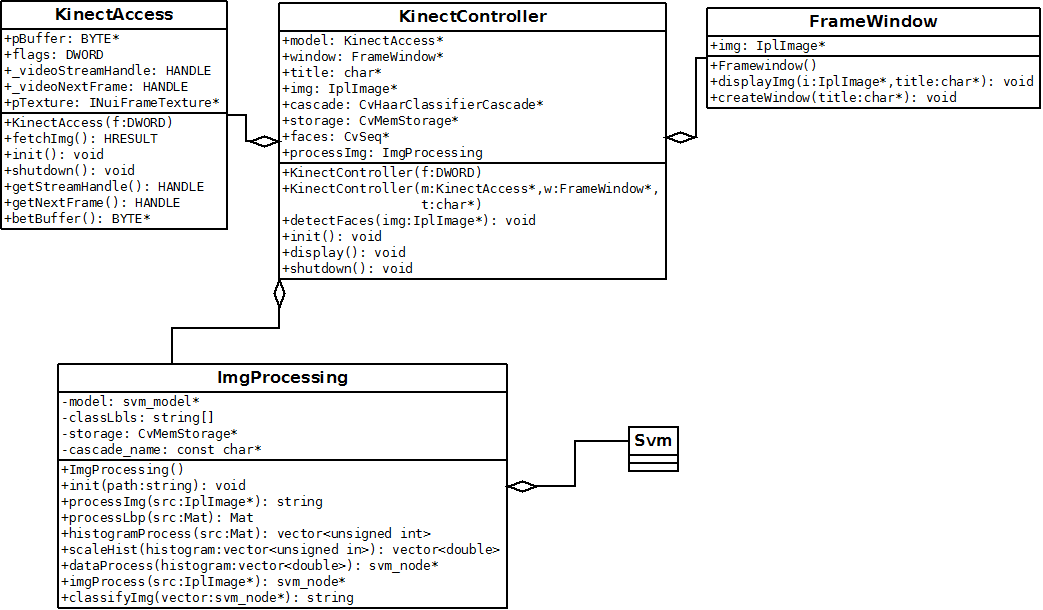
\includegraphics[scale=0.3]{figures/UML} 
\newline
\caption{UML diagram describing our implementation of a facial expression recognition system}
\label{uml}
\end{center} 
\end{figure}

\phantomsection
\section{Interactions}

\vspace{\baselineskip}
\noindent There are two possible ways for the user to interact with the system:
\begin{itemize}
  \item The user has to show a facial expression in front of the camera;
  \item The user has to decide when he or she wants the program to perform facial expression recognition.
\end{itemize}

\noindent The first possibility does not need the user to be active. Indeed, the Kinect camera sensor can record 30 images per second, so each expression can be caught in the image stream. That is why the second possibility needs to be trigged by the user (in our case, press a button) to "capture" the facial expression and start the analysis process. 

\phantomsection
\section{Algorithm}
\vspace{\baselineskip}

\noindent The entry point of the software first initializes the 3 MVC modules. It then runs 3 functions through the controller:

\begin{itemize}
  \item Initialization which loads models (for face detection and classification through SVM) and begins images capture;
  \item Main loop of the program which displays images and waits for actions from the user;
  \item Shutdown process, which deletes models, releases memory and closes communication with sensors.
\end{itemize}

\fbox{
\begin{minipage}{0.7\textwidth}
   \textbf{Main loop algorithm} 

\begin{algorithmic}
\While{button 'q' is not pressed} 
	\State wait for single object from videoNextFrame handle
	\State result $\gets$ fetchImage(videoStream handle)
	\If{result == success}
		\State Texture $\gets$ Image.texture
		\State LockedRectangle $\gets$ Texture.lockedRectangle
		\If{LockedRectangle.bits $\neq$ 0}
			\State buffer $\gets$ LockedRectangle.bits
			\State unlockRectangle()
			\State releaseImageFrame(videoStream handle)
			\State openCvImage $\gets$ buffer
			\State face $\gets$ detectFace(openCvImage)
			\State roi $\gets$ setRegionOfInterest(face)
			\If{button 'r' is pressed}
				\State openCvImage2 $\gets$ openCvImage
				\State greyscImage $\gets$ convertToGrayscale(openCvImage2)
				\State featVector $\gets$ lbpProcess(greyscIimage)
				\State label $\gets$ classify(featVector)
				\State display(label)
			\EndIf
			\State delete(roi)
		\EndIf
	\EndIf
\EndWhile
\end{algorithmic}
\end{minipage}
}


